%!TEX TS-program = xelatex
\documentclass[a4paper,14pt]{article}
\usepackage[utf8]{inputenc}
\usepackage[T1]{fontenc}

%%% Работа с русским языком
\usepackage[english,russian]{babel}   %% загружает пакет многоязыковой вёрстки
\usepackage{fontspec}      %% подготавливает загрузку шрифтов Open Type, True Type и др.
\defaultfontfeatures{Ligatures={TeX},Renderer=Basic}  %% свойства шрифтов по умолчанию
\setmainfont[Ligatures={TeX,Historic}]{Times New Roman} %% задаёт основной шрифт документа
\setsansfont{Comic Sans MS}                    %% задаёт шрифт без засечек
\setmonofont{Courier New}
\usepackage{indentfirst}
\frenchspacing

\renewcommand{\epsilon}{\ensuremath{\varepsilon}}
\renewcommand{\phi}{\ensuremath{\varphi}}
\renewcommand{\kappa}{\ensuremath{\varkappa}}
\renewcommand{\le}{\ensuremath{\leqslant}}
\renewcommand{\leq}{\ensuremath{\leqslant}}
\renewcommand{\ge}{\ensuremath{\geqslant}}
\renewcommand{\geq}{\ensuremath{\geqslant}}
\renewcommand{\emptyset}{\varnothing}

%%% Дополнительная работа с математикой
\usepackage{amsmath,amsfonts,amssymb,amsthm,mathtools} % AMS
\usepackage{icomma} % "Умная" запятая: $0,2$ --- число, $0, 2$ --- перечисление

%% Номера формул
%\mathtoolsset{showonlyrefs=true} % Показывать номера только у тех формул, на которые есть \eqref{} в тексте.
%\usepackage{leqno} % Нумерация формул слева	

%% Перенос знаков в формулах (по Львовскому)
\newcommand*{\hm}[1]{#1\nobreak\discretionary{}
{\hbox{$\mathsurround=0pt #1$}}{}}

%%% Работа с картинками
\usepackage{graphicx}  % Для вставки рисунков
\graphicspath{{images/}}  % папки с картинками
\setlength\fboxsep{3pt} % Отступ рамки \fbox{} от рисунка
\setlength\fboxrule{1pt} % Толщина линий рамки \fbox{}
\usepackage{wrapfig} % Обтекание рисунков текстом

%%% Работа с таблицами
\usepackage{array,tabularx,tabulary,booktabs} % Дополнительная работа с таблицами
\usepackage{longtable}  % Длинные таблицы
\usepackage{multirow} % Слияние строк в таблице
\usepackage{float}% http://ctan.org/pkg/float

%%% Программирование
\usepackage{etoolbox} % логические операторы


%%% Страница
\usepackage{extsizes} % Возможность сделать 14-й шрифт
\usepackage{geometry} % Простой способ задавать поля
\geometry{top=20mm}
\geometry{bottom=20mm}
\geometry{left=20mm}
\geometry{right=10mm}
%
%\usepackage{fancyhdr} % Колонтитулы
% 	\pagestyle{fancy}
%\renewcommand{\headrulewidth}{0pt}  % Толщина линейки, отчеркивающей верхний колонтитул
% 	\lfoot{Нижний левый}
% 	\rfoot{Нижний правый}
% 	\rhead{Верхний правый}
% 	\chead{Верхний в центре}
% 	\lhead{Верхний левый}
%	\cfoot{Нижний в центре} % По умолчанию здесь номер страницы

\usepackage{setspace} % Интерлиньяж
\onehalfspacing % Интерлиньяж 1.5
%\doublespacing % Интерлиньяж 2
%\singlespacing % Интерлиньяж 1

\usepackage{lastpage} % Узнать, сколько всего страниц в документе.

\usepackage{soul} % Модификаторы начертания

\usepackage[hyphens]{url}
\usepackage{hyperref}
\usepackage[usenames,dvipsnames,svgnames,table,rgb]{xcolor}
\hypersetup{                % Гиперссылки
    unicode=true,           % русские буквы в раздела PDF
    pdftitle={Детекция объектов по нескольким примерам без дообучения},   % Заголовок
    pdfauthor={Самоделкина М.В., Подчезерцев А.Е.},      % Автор
    pdfsubject={Детекция объектов по нескольким примерам без дообучения},      % Тема
    pdfcreator={Самоделкина М.В., Подчезерцев А.Е.}, % Создатель
    pdfproducer={Самоделкина М.В., Подчезерцев А.Е.}, % Производитель
%    pdfkeywords={keyword1} {key2} {key3}, % Ключевые слова
    colorlinks=true,        % false: ссылки в рамках; true: цветные ссылки
    linkcolor=black,          % внутренние ссылки
    citecolor=black,        % на библиографию
    filecolor=magenta,      % на файлы
    urlcolor=black           % на URL
}
\makeatletter
\def\@biblabel#1{#1. }
\makeatother
\usepackage{cite} % Работа с библиографией
%\usepackage[superscript]{cite} % Ссылки в верхних индексах
%\usepackage[nocompress]{cite} % 
\usepackage{csquotes} % Еще инструменты для ссылок

\usepackage{multicol} % Несколько колонок

\usepackage{tikz} % Работа с графикой
\usepackage{pgfplots}
\usepackage{pgfplotstable}

\usepackage{ dsfont }

\newcommand{\imref}[1]{рис.~\ref{#1}}

\usepackage{multirow}
\usepackage{spreadtab}
\newcolumntype{K}[1]{@{}>{\centering\arraybackslash}p{#1cm}@{}}


\usepackage{xparse}
\usepackage{fancyvrb}

\RecustomVerbatimCommand{\VerbatimInput}{VerbatimInput}
{
    fontsize=\footnotesize
}

\newcolumntype{?}[1]{!{\vrule width #1}}

\usepackage{tocloft}
\renewcommand{\cftsecleader}{\cftdotfill{\cftdotsep}}

\usepackage{pdfpages}

\usepackage{rotating}

\usepackage{pdflscape}

\usepackage{ragged2e}
\usepackage{microtype}

\usepackage{subcaption}

% Выравнивание по ширине без переносов слов
\justifying
\sloppy
\tolerance=500
\hyphenpenalty=10000
\emergencystretch=3em

% Подогнать таблицу под ширину страницы
\usepackage{adjustbox}

\usepackage{titlesec}

% ГОСТ заголовки таблицы
\usepackage[font=small]{caption}

\captionsetup[figure]{justification=centering,labelsep=period} % Картинки по центру, с точкой после рис

\DeclareCaptionLabelFormat{rightline}{\rightline{\bothIfFirst{#1}{ }#2}}
%\captionsetup[table]{justification=centering,labelformat=rightline,labelsep=newline}
\captionsetup[table]{justification=raggedleft,labelformat=rightline,labelsep=newline}

\newcommand{\tablecaption}[1]{\addtocounter{table}{1}\small \begin{flushright}
                                                                \tablename \ \thetable
\end{flushright}%
    \begin{center}
        #1
    \end{center}}

\usepackage{enumerate}

%сноска с новым номером на кждоый странице
\usepackage[perpage]{footmisc}
\usepackage[fixlanguage]{babelbib}
\usepackage{lastpage}
\begin{document}

    \begin{titlepage}
    \begin{center}
        ПРАВИТЕЛЬСТВО РОССИЙСКОЙ ФЕДЕРАЦИИ \\
        ФЕДЕРАЛЬНОЕ ГОСУДАРСТВЕННОЕ АВТОНОМНОЕ \\
        ОБРАЗОВАТЕЛЬНОЕ УЧРЕЖДЕНИЕ ВЫСШЕГО ОБРАЗОВАНИЯ\\
        «НАЦИОНАЛЬНЫЙ ИССЛЕДОВАТЕЛЬСКИЙ УНИВЕРСИТЕТ\\
        «ВЫСШАЯ ШКОЛА ЭКОНОМИКИ»
    \end{center}

    \begin{center}
        \textbf{Факультет компьютерных наук}

        \textbf{Образовательная программа <<Финансовые технологии и анализ данных>>}

%        \vspace{2ex}

    \end{center}
    \vspace{1ex}

    \begin{center}
        \textbf{Курсовая работа \\
            <<Детекция объектов по нескольким примерам без дообучения>>
        }
    \end{center}

    \vspace{2ex}
    \vfill

    \vspace{2ex}

    \begin{flushright}
        \textbf{Выполнили:}

        \vspace{2ex}

        Студенты группы мФТиАД21

        \vspace{2ex}

        Самоделкина Мария Владимировна

        Подчезерцев Алексей Евгеньевич

        \vspace{2ex}
        \textbf{Руководитель:}

        Приглашенный преподаватель

        Озерин Алексей Юрьевич

    \end{flushright}

    \vspace{5ex}
    \begin{center}
        Москва \the\year \, г.
    \end{center}

\end{titlepage}
\addtocounter{page}{1}

    \section*{\normalsize \hfill Аннотация \hfill}

    ...

    \sloppy
    \newpage

    \section*{\normalsize \hfill Abstract \hfill}

    ...

    \newpage

    \tableofcontents
    \pagebreak

    \section*{Введение}
    \addcontentsline{toc}{section}{\protect\numberline{}Введение}


    \newpage


    \section{Теоретическая часть}

    \subsection{Основные понятия}

    Задача детекции объектов (object detection) на изображении включает в себя несколько подзадач:
    \begin{enumerate}
        [1)]
        \itemsep0em
        \item определение прямоугольной области, ограничивающей объект (bounding box, bbox);
        \item классификация выделенной области;
    \end{enumerate}
    В результате работы модели, решающей задачу поиска объектов, получаются области или регионы изображения (object proposals) в которых может находиться объект, а также определена вероятность принадлежности этого объекта к определенному классу.

    Дополнительно могут решаться задачи нахождения ключевых точек объекта и сегментации - отделения объекта от фона, нахождение маски объекта.

    Наиболее популярные датасеты для обучения модели детекции объектов: MS~COCO~\cite{COCO}, LVIS~\cite{LVIS}, Objects365~\cite{Objects365}.
    Датасет LVIS содержит 164 тысячи изображений для решения задачи сегментации. Разработчиками предоставлена высококачественная разметка для более 1200 различных категорий.
    % TODO как оценивают качество в lvis по категориям
    
    Эмбеддинг (embedding) -- скрытое векторное представление объекта (текстовых, графические, табличных и аудио данных) фиксированной размерности.

    Карта признаков (feature map) -- векторное представление изображения нефиксированной размерности, где элемент карты содержит информацию о некоторой области изображения.

    NMS (non-maximum suppression)~\cite{neubeck2006efficient} -- алгоритм выделения регионов изображения с максимумом уверенности в классификации.
    В данном алгоритме объединяются регионы, отношение площади пересечения к объединению (IoU, Intersection over Union) которых больше заданного порога.
    Алгоритм позволяет получить из большого числа похожих или маловероятных регионов изображений один или несколько малопересекающихся регионов.

	\subsection{Модели для решения задачи детекции объектов}

    Mask R-CNN (Regions With CNNs)~\cite{MaskRCNN} -- двухэтапная нейронная сеть, позволяющая решать задачи детекции объектов и сегментации. В основе сети лежит сверточная нейронная сеть FCN (Fully Convolutional Network), состоящая только из сверточных (convolution) слоев и слоев подвыборки (pooling). Первый модуль RPN (Region Proposal Network) позволяет выделить регионы изображения по карте признаков сверточной нейронной сети. Вторым этапом происходит предсказание bounding box, класса и маски объекта для каждого региона.

    YOLO (You Only Look Once)~\cite{redmon2016you} -- семейство архитектур моделей, позволяющее ускорить решение задачи детекции объектов и получать результаты в режиме реального времени.
    Это одноэтапная нейронная сеть, не использующая модуль для выделения регионов изображения.
    В модели сначала получают карты признаков для изображения с помощью сверточных слоев (backbone часть), далее для каждого элемента карты решаются задачи определения класса объекта и его размеров, центр которого находится в данном элементе карты (head часть).
    В модели используется 3 карты признаков различных размеров: каждая последующая получается применением набора сверток к предыдущей.
    Такой подход используется для нахождения объектов разных размеров -- маленьких, средних и больших.
    Модели YOLO обучены на датасете COCO, содержащем 80 категорий.

    CLIP (Contrastive Language–Image Pre-training)~\cite{CLIP} -- модель, позволяющая переводить текстовые описания и изображения в единое векторное пространство.
    CLIP предоставляет возможность решать задачу детекции объектов без дообучения для произвольных классов.
    В основе модели лежат Text Encoder и Image Encoder для преобразования текста и изображения в векторные представления, косинусное расстояние между которыми максимизируется для релевантных пар текста и изображения и минимизируется для нерелевантных.
    
    \subsection{Приблизительный поиск ближайших соседей}
    
    Для поиска похожих эмбеддингов среди набора заранее заданных эмбеддингов используют методы приблизительного поиска ближайших соседей.
    Такие алгоритмы позволяют ускорить поиск, по сравнению с полным перебором всех объектов, однако требуют дополнительных затрат на построения индекса, 
    могут возвращать не самых ближайших соседей, а только приближенных к ним.
    В основе таких методов лежат алгоритмы вероятностного хеширования~\cite{tao2010efficient}, которые проецируют похожие объекты в одинаковые корзины, после этого осуществляется поиск ближайших соседей среди объектов корзины;
    деревев поиска~\cite{liu2006new}, которые разделяют все пространство на небольшие подпространства и проводят поиск среди части объектов в подпространстве;
    построение графов~\cite{malkov2018efficient}, где вершинами являются исходные эмбеддинги, а 
    ребра ~--~ связи между близкими вершинами, поиск кандидатов осуществляется жадным блужданием по графу.
    Различные комбинации и оптимизации алгоритмов построения индекса и поиска позволяют дополнительно сократить время поиска объекта или повысить точность результатов~\cite{annoy,avq_2020}.
    
    \subsection{Выводы к главе \thesection}
    \begin{enumerate}
    	[1)]
    	\itemsep0em
    	\item йцу
    \end{enumerate}
    
    \newpage
    
 	\section{Обзор литературы}

    \subsection{Детекция объектов по произвольному текстовому запросу}

    В статье~\cite{ViLD} предложен метод ViLD - Vision and Language knowledge Distillation, позволяющий находить объекты с произвольным текстовым описанием.
    На этапе обучения рассчитываются текстовые эмбеддинги описаний категорий и эмбеддинги регионов изображения с использованием предобученной модели (модель-учитель).
    Обучается модель детекции объектов Mask R-CNN (модель-ученик), которая дополнительно максимизирует расстояние между эмбеддингом региона предобученной модели-учителя и эмбеддингами региона модели-ученика.
    Таким образом, происходит извлечение знаний (дистилляция) из модели-учителя.
    Во время применения модели-ученика предобученная модель-учитель используется только для получения текстовых эмбеддингов, а эмбеддинги для регионов получается из модели-ученика.
    Итоговые регионы получаются в результате ранжирования оценок, полученных как скалярное произведение текстового эмбеддинга модели-учителя и эмбеддинга региона модели-ученика.

    В качестве модели-учителя в статье используется модель CLIP.
    Модель обучена на датасете LVIS. 
    В работе отмечается, что модель может применяться и к другим датасетам (COCO, Objects365) без дообучения.

    Преимуществом описанного подхода является использование одной модели как для выделения регионов, так и для получения их эмбеддингов, что ускоряет время применения, однако точность при таком подходе понижается.

    Полученную модель предлагается использовать следующим образом: для изображения подавать набор текстовых описаний и отбирать заданное количество регионов с минимальным скалярным произведением.

    К недостаткам предлагаемого подхода можно отнести поиск текстовых описаний только на одном изображении, то есть при отсутствии объектов, релевантных набору текстовых описаний, алгоритм выведет требуемое количество регионов (для нерелевантных текстовых описаний скалярное произведение также может быть высокое).

    \subsection{Простая детекция объектов по нескольким примерам}

    В работе~\cite{wang2020few} авторы предлагают двушаговый алгоритм дообучения моделей для детекции на нескольких примерах.
    Кроме того, используются метрики качества, оценивающие качество работы модели на популярных или на редких изображениях.
    Авторы используют несколько датасетов -- COCO, LVIS и PASCAL VOC,
    и несколько архитектур моделей -- Faster R-CNN, VGG16, YOLOv2, для проверки своих гипотез.
    На первом этапе обучается модель на объектах, классы которых часто встречаются в выборке.
    На следующем этапе предлагается заморозить все веса сети, кроме последнего, и обучать модель на выборке, состоящей из частых и редких объектов в равных пропорциях.
    Такой подход позволил повысить качество работы моделей на несколько пунктов, в зависимости от датасета и модели.
    
    %TODO статья

    \subsection{Инженерный подход к разметке изображений}

    В решении~\cite{AnnoMage} реализован подход для полу-автоматизированной разметки датасетов изображений. 
    В предложенном приложении автоматически размечаются области, соответствующие выбранным классам датасета COCO, полученные с помощью загруженной модели.

    В отличие от решения ~\cite{AnnoMage} в курсовой работе предлагается подход с дообучением модели на новой разметке и применением модели для произвольных текстовых запросов.

    \subsection{Цель и задачи исследования}
    
    Предлагаемый подход можно применять также для отбора наиболее релевантных изображений из пользовательского датасета.

    Задачи:
    \begin{enumerate}
        [1)]
        \itemsep0em
        \item йцу

    \end{enumerate}

    \subsection{Выводы к главе \thesection}
    \begin{enumerate}
        [1)]
        \itemsep0em
        \item йцу
    \end{enumerate}

    \newpage


    \section{Практическая часть}
    
	\subsection{Описание данных}    
	%TODO Более подробно про датасет LVIS, какие категории, сколько редких
    
    \subsection{Подход к детекции объектов по произвольному текстовому запросу}
    
    Целью данного подхода является выделение заданного количества наиболее релевантных изображений по произвольному текстовому описанию. 
    Подход реализуется в несколько этапов:
     \begin{enumerate}
    	[1)]
    	\itemsep0em
    	\item получение регионов для всего доступного множества изображений;
    	\item вычисление векторного представления регионов и текстового запроса;
    	\item поиск ближайших регионов к текстовому запросу.
    \end{enumerate}
    
    При проведении эксперимента для оценки качества предлагаемого подхода используются изображения датасета LVIS. 
    
    В качестве модели для выделения регионов использовалась одноэтапная модель YOLOv5. 
    Исходная модель YOLOv5 была модифицирована таким образом, чтобы в результате применения модели получалось как можно больше регионов. 
    Для этого уменьшался порог уверенности модели в классификации и для объединения похожих регионов использовался модифицированный алгоритм NMS. 
    
    В измененном алгоритме NMS не учитывается предсказанный класс объекта ~--~ это сделано для того, чтобы получать регионы  для объектов, на которые модель не была обучена. 
    Чтобы избавиться от дублированных регионов к ограничивающей области была применена кластеризация методом k-средних с заданным максимальным количеством классов, после чего к областям одного класса применялся классический алгоритм NMS. 
    На рис.~\ref{fig:nms} продемонстрирован результат работы модифицированного алгоритма NMS: результат кластеризации дублированных регионов представлен на рис.~\ref{fig:nms1}, кластера отмечены одним цветом; итоговый результат применения NMS к выделенным кластерам изображен на рис.~\ref{fig:nms2} ~--~ количество выделенных регионов существенно уменьшено.
    
    \begin{figure}[H]
    	\centering
    	\begin{subfigure}{.5\textwidth}
    		\centering
    		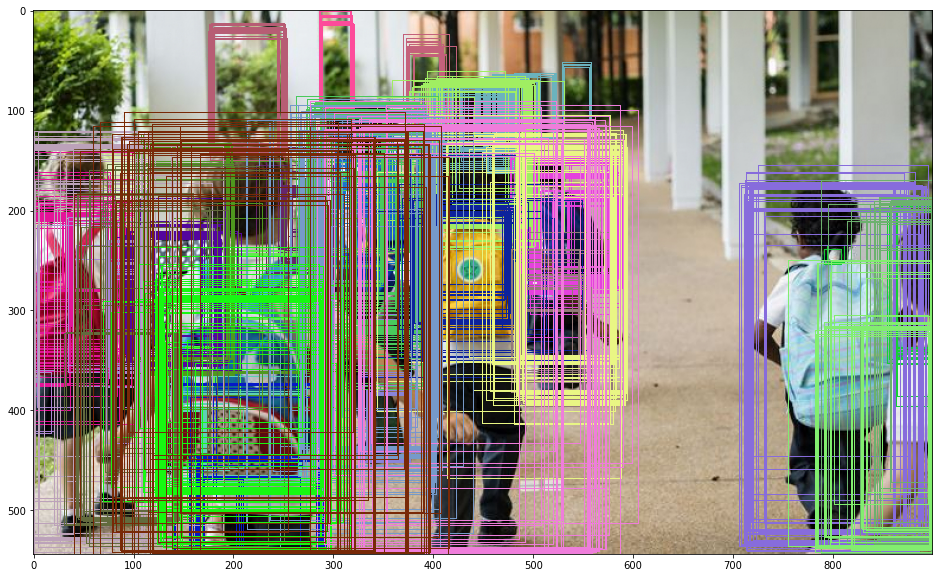
\includegraphics[width=\linewidth]{images/before_nms}
    		\caption{Результат кластеризации регионов}
    		\label{fig:nms1}
    	\end{subfigure}%
    	\begin{subfigure}{.5\textwidth}
    		\centering
    		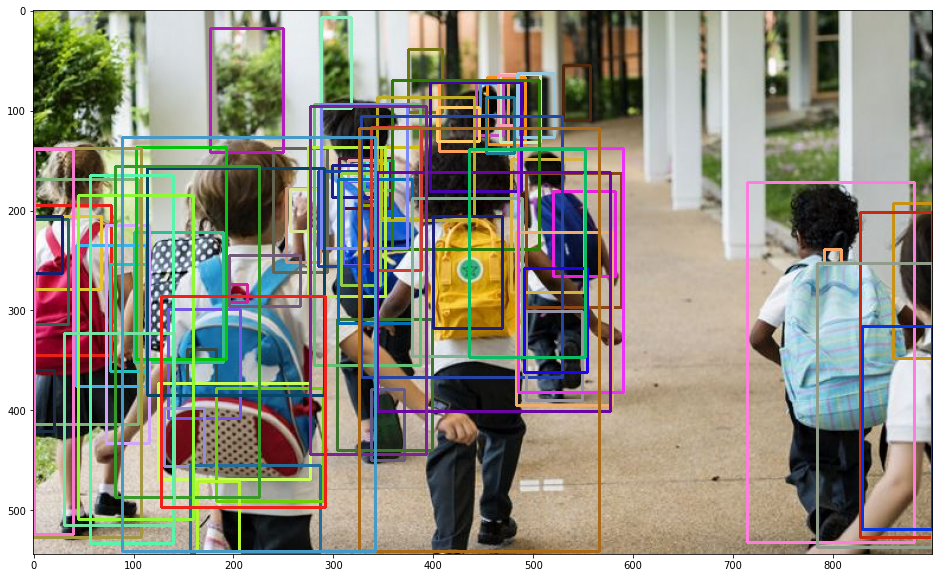
\includegraphics[width=\linewidth]{images/after_nms}
    		\caption{Результат применения NMS к кластерам}
    		\label{fig:nms2}
    	\end{subfigure}
    	\caption{Демонстрация работы модифицированного алгоритма NMS}
    	\label{fig:nms}
    \end{figure}
    
    При проведении эксперимента количество кластеров для метода k-средних определялось по следующей формуле:
    $\max(\min(30, \left[\frac{m}{2}\right]), 1),$ где $m$~--~количество найденных на изображении регионов. 
    Для проведения расчетов использовались также следующие гиперпараметры:
    \begin{center}
    	\begin{tabular}{| l | l |}
    		\hline
    		Порог уверенности модели в классификации & 0.01\\ \hline
    		Пороговое значение IoU & 0.45 \\ \hline
    		Максимальное количество регионов в NMS  & 10\\
    		\hline
    	\end{tabular}
    \end{center}

	Далее для каждого выделенного региона изображения применялась модель CLIP. 
	Текстовый запрос также переводился в векторное пространство с помощью этой модели. 
	Для тестирования подхода в качестве текстовых запросов использовались определения категорий датасета LVIS.
	
	С помощью приблизительного поиска ближайших соседей, а также полным перебором по максимизации косинусного расстояния для сравнения результатов осуществлялся поиск заданного количества ближайших векторов регионов к вектору текстового запроса (определению категории).
	
	%TODO В результате применения подхода исследовались следующие метрики
    
    Таким образом, для повышения точности среди выбранных изображений в предлагаемом подходе последовательно используются 2 модели.
    
    В качестве эксперимента также было проведено сравнение качества модели ViLD при использовании только результатов выделения регионов, а также с использованием эмбеддинга региона из модели ViLD. 
    В последнем случае модель CLIP не применялась к найденным регионам.
    %TODO провести такой эксперимент
    
    \subsection{Решение задачи регрессии ключевых точек с дообучением по нескольким примерам}
    
    В курсовой работе исследован подход к решению задачи регрессии ключевых точек с дообучением по нескольким примерам. 
    Задача решается в несколько этапов:
     \begin{enumerate}
    	[1)]
    	\itemsep0em
    	\item получение карты признаков для входящего набора изображений с помощью предобученной модели;
    	\item обучение нескольких моделей линейной регрессии для нахождения каждой ключевой точки.
    \end{enumerate}
	При проведении эксперимента в качестве предобученной модели использовались YOLOv5 и Fast R-CNN ~--~ двухэтапная модель для решения задачи детекции объектов из библиотеки Detectron2. 
	На рис.~\ref{fig:stage9_SPPF_features} представлена визуализация элементов последнего слоя backbone части модели YOLOv5.
	\begin{figure}[H]
		\centering
		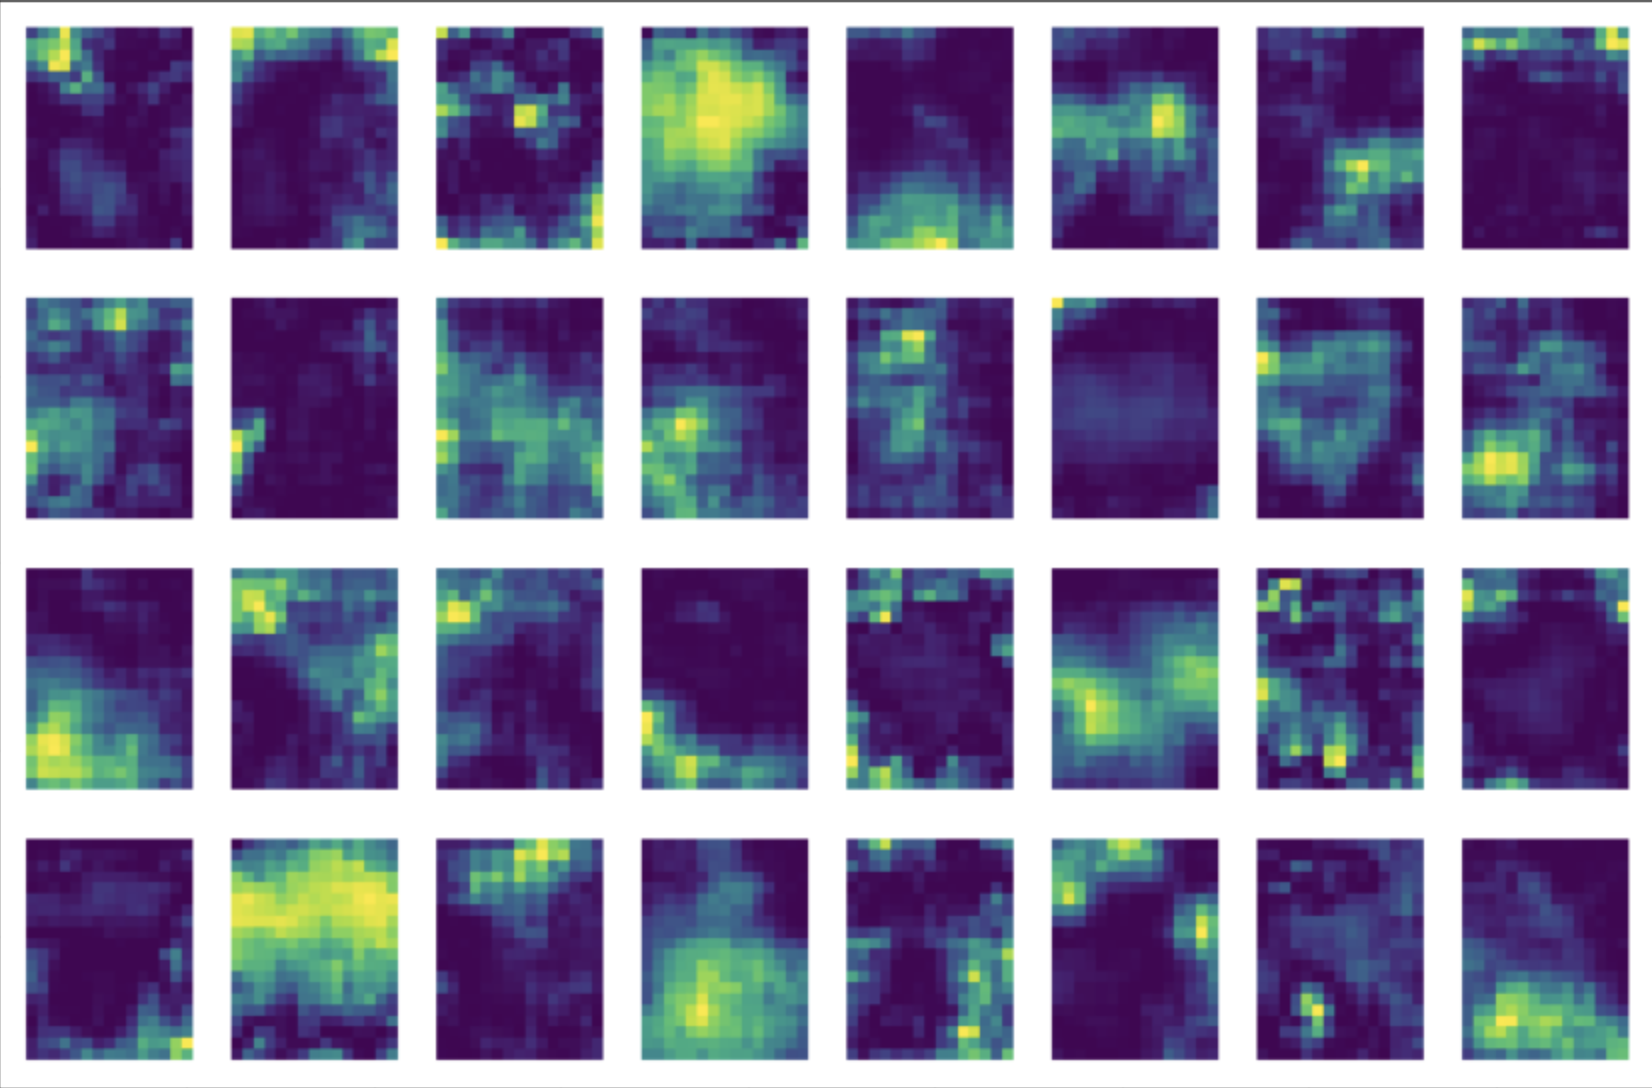
\includegraphics[width=0.7\linewidth]{images/stage9_SPPF_features}
		\caption{Визуализация элементов последнего слоя backbone части модели YOLOv5}
		\label{fig:stage9_SPPF_features}
	\end{figure}
	
	В качестве признаков для модели регрессии выбирался центральный вектор карты признаков и еще 8 ближайших к нему векторов. 
	Положение центрального вектора карты признаков определяется формулой $x_c =\left[\left( [\frac{w}{s}]+1\right) \cdot 0.5\right],$ где $w$ ~--~ размер изображения, $s$ ~--~ размер элемента карты признаков.
	Для каждого из 9 векторов-признаков значение ключевой точки пересчитывалось с учетом расположения данного вектора относительно центра по формуле $x' = \frac{x}{s} - (x_v + 0.5)$, где $x$ ~--~ ключевая точка, $x_v$ ~--~ положение вектора-признака
	
	Во время применения подхода для нахождения каждой ключевой точки использовались 9 векторов-признаков, а в качестве предсказания бралось среднее значение всех 9 прогнозов линейной регрессии на векторах-признаках. 
	Преобразование предсказания модели в значение ключевой точки осуществлялось по формуле $x_p = (x'_p +  x_c) * s$, где $x'_p$ - предсказание модели.
    
    Однако данный подход не показал качественного результата.
    %TODO метрики качества для регрессии или картинка с котиками
    % TODO добавить аугментации
    
    \subsection{Алгоритм улучшения результатов выдачи}
    
    Предобученные модели могут не выделять или выделять некачественно интересующие пользователя объекты.
    Для решения этой проблемы был реализован алгоритм по улучшению результатов выдачи пайплайна по выделению регионов изображения.
    
    Была добавлена возможность выбора картинок, которые соответствуют пользовательскому запросу, указанию нерелевантных или загрузки пользовательских изображений, содержащих заданные объекты.
    После пользователь может или оставить предложенные регионы для выбранных изображений, или скорректировать их.
    Далее на полученной разметке выполняется дообучение модели выделения регионов.
    В случае малого количества наблюдений может быть произведена заморозка части весов сети~\cite{wang2020few}.
    Полученную модель можно использовать как самостоятельную для поиска регионов изображений, соответствующим интересующим объектам, так и для повторного запуска на выборке и создания новой модели для поиска по текстовому запросу.
    
    \subsection{Демонстрация результатов работы предложенного алгоритма детекции объектов}
    
    Про демо в ноутбуке и демо сайтик: какие функции, какие классы, какой функционал, как реализовано (либа)
    
    \subsection{Результаты экспериментов}
    
    \subsubsection{Поиск ближайших соседей}
    
    Для оценки качества алгоритмов поиска ближайших соседей был проведен эксперимент.
    В качестве поисковой базы использовались эмбеддинги областей изображений, полученные для валидационной выборки датасета LVIS с помощью регионов модели YOLOv5 и эмбеддингов CLIP, в выборке~852831 наблюдений, размерность эмбеддинга~512.
    Для текстовых запросов использовались эмбеддинги для определений классов датасета LVIS, в качестве модели для получения эмбеддингов выступал CLIP, в выборке~1203 наблюдений.
    В качестве меры близости использовалось косинусное сходство.
    Стоит отметить, что особенность такого датасета ~--~ относительно низкое значение схожести для наиболее близких векторов.
    Так, значение метрики около~0,3 соответствует хорошей схожести и на реальных запросах редко оказывается значительно выше этого порога.
    
    Для подсчета качества алгоритмов поиска ближайших соседей использовалась метрика Recall~\cite{aumuller2020ann}. 
    В качестве истинных ответов к запросу брались ближайшие к текстовому запросу 30 областей изображений, полученные с помощью полного перебора.
    Количество правильных ответов алгоритма получались как пересечение объектов, выданных алгоритмом (до 30), и истинных ответов. 
    Метрика для одного текстового запроса получалась как доля правильных ответов алгоритма.
    Итоговая метрика усреднялась по всем текстовым запросам.
    
    Для тестирования были выбраны библиотеки Annoy~\cite{annoy}, ScaNN~\cite{avq_2020}, Hnswlib (NMSLIB)~\cite{malkov2018efficient}, а также полный перебор.
    В алгоритме Annoy происходил подбор количества деревьев, которые разделяют пространство признаков.
    В алгоритме ScaNN происходил подбор количества листьев, доли листьев, используемых в итоговом поиске, количество кандидатов, для которых будет произведен точный расчет расстояния до заданного вектора.
    В алгоритме Hnswlib подбиралось количество ребер для каждой вершины, сложность построения графа, способ постобработки результатов.
    
    Тестирование проводилось на виртуальной машине с~32 vCPU Intel Xeon Processor (Icelake), 64ГиБ оперативной памяти, Ubuntu~20.04.3~LTS, Python~3.8.10.
    
    На графике~\ref{fig:ann_recall_qps} представлена зависимость метрики Recall от скорости алгоритма (количества запросов в секунду).
    Различное количество запросов для одного алгоритма обусловлено перебором гиперпараметров, влияющих на скорость и точность. 
    Красной точкой на графике отмечен полный перебор ~--~ он имеет идеальную точность (с помощью него осуществлялся выбор правильных ответов), но наиболее медленное время выполнения.
    Можно сделать вывод, что на исследуемом наборе данных алгоритм Annoy работает хуже алгоритмов ScaNN и NMSLib и по скорости, и по точности. 
    Наиболее быстрым является алгоритм NMSLib, наиболее точным ~--~ ScaNN.
    
    \begin{figure}[H]
    	\centering
    	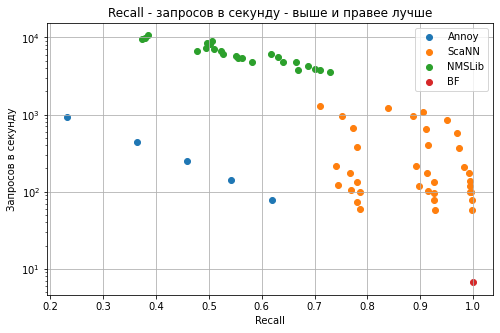
\includegraphics[width=0.7\linewidth]{images/ann_recall_qps}
    	\caption{Recall - запросов в секунду - выше и правее лучше}
    	\label{fig:ann_recall_qps}
    \end{figure}

	На рис.~\ref{fig:ann_recall_build} представлен анализ времени построения индекса алгоритма и точности. 
	Алгоритм ScaNN имеет наименьшее время построения индекса, а ScaNN и NMSLib примерно одинаковое, в зависимости от параметров модели.

    \begin{figure}[H]
		\centering
		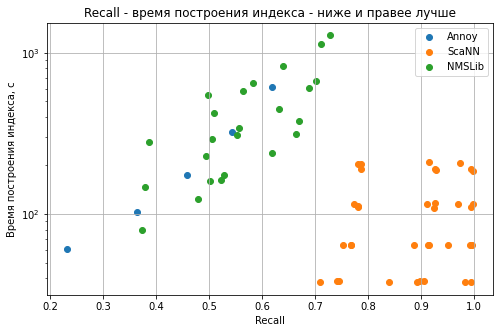
\includegraphics[width=0.7\linewidth]{images/ann_recall_build}
		\caption{Recall - время построения индекса - ниже и правее лучше}
		\label{fig:ann_recall_build}
	\end{figure}

    \subsection{Рекомендации по использованию полученных результатов}
    
    На какие грабли наступили и что не стоит использовать
    
    annoy не работает
    
    подход с kpoints - дообучение не работает
    
    какой подход лучше yolo или vild (дообучать модели или нет)
    
    зашел подход с раскручиванием nms
    
    как в итоге использовать полученную демку (для сбора датасета, для отбора изображений с пользовательского датасета)
    
    что стоит доработать в демке, что стоит попробовать из моделей, из подходов (+ эксперименты kpoints, что стоит использовать вместо полного перебора, более современные архитектуры (новая статья))
       
    \subsection{Выводы к главе \thesection}
    \begin{enumerate}
        [1)]
        \itemsep0em
        \item йцу
    \end{enumerate}

    \newpage


    \section{Заключение}

    В работе изучена...

    \newpage
    \renewcommand{\refname}{{\normalsize \hfill Список использованных источников \hfill}}
%    \bibliographystyle{unsrt}
    \selectbiblanguage{russian}
    \bibliographystyle{BibTeX-Styles/ugost2008mod}
    \bibliography{main}
    \newpage

\end{document}